\setlength{\footskip}{8mm}

\chapter{Introduction}

\textit{This chapter provides some background information on this project and the objectives that are to be achieved.}

\section{Background}
Beginning from the late 2000s, commercial unmanned aerial vehicles (UAVs) became more widespread as they became cheaper and more accessible to the general public. The first and most obvious implementation of UAVs was in the military. Military drones – both aerial and non-aerial – have been widespread since the late 20th century but it was not until very recently that UAVs have been successfully commercialized, as is obvious in the examples mentioned in the next paragraph. 

Companies are finding more and more innovative ways to commercialize drones. For example, Zipline uses fixed-wing drones to deliver essential medical supplies in rural Rwanda. Ele.me is a meal delivery service in Shanghai, China that plans to distribute meal packages in Shanghai\textquotesingle s industrial park. Amazon Prime Air is also another logistical delivery service currently in development by the tech giant. Aside from commercial applications, UAVs can also be used in the industrial, agricultural, scientific sectors. The FAA in the United States predicts that the number of commercial drones in the US will grow tenfold over the next five years, from 42,000 in 2016 to more than 420,000 in 2021\cite{faa}. 

The vast majority of UAVs – with the exception of UAVs with AIs – are supported by a ground controller. This ground controller sends commands to the onboard flight controller by some standardized communication protocol. The flight controller usually has some form of autopilot that accepts commands through this protocol.
In this study, the terms ‘UAV’ and ‘drone’ will be interchangeably and will be the same meaning. All terrestrial non-aerial drones are excluded in the context of this study.


% \begin{figure}[t]
%   \centering
%   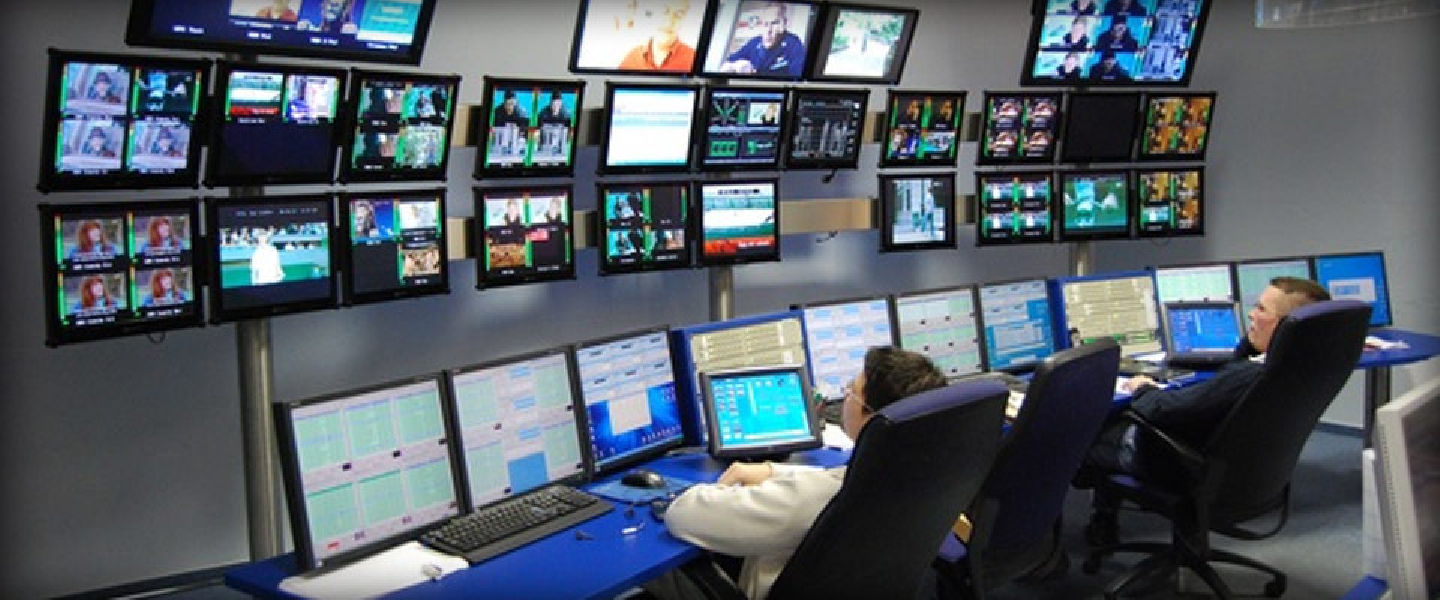
\includegraphics[width=5in]{figures/monitoring}
%   \caption[CCTV monitoring room.]{\small CCTV monitoring
%     room. Reprinted from the Twenty First Security Web site
%     (\url{http://www.twentyfirstsecurity.com.au/}).}
%   \label{fig:monitoring}
% \end{figure}

\section{Problem Statement}

However, for UAVs to be utilized effectively and to their full potential, drones need to be automated, instead of manually controlled by operators, as in the case of most military drones. Users should only have to input basic data, such as flight data. For this reason, a web interface to command and control a fleet of drones is necessary, so that commands can be sent from anywhere. 

Since the ground controller is a web application, it will not be wholly similar to a normal ground station controller. Data, i.e. flight parameters, from the user has to be processed and then sent first to the onboard computer, which will then send them through a protocol to the flight controller.

Standardized protocols such as MAVLink already exist, but these have to be either supplemented or supplanted by another form of communication due to the web automation element. One form may be a remote-procedure call (RPC) protocol to call functions on the UAV\textquotesingle s onboard computer. 
s
SSH is an effective way to access the onboard computer securely but this is complicated by the dynamic network presence of the drone, i.e. a dynamic IP, since it is connected to the web through an LTE module. This can be addressed by use of a reverse SSH tunnel with port forwarding from the drone, as a means of punching through the NAT used by the LTE SIM card. This will be explained further in Chapter \ref{ch:methodology}.

The problem to be resolved is for the communication process all the way from the user to the controller to be as streamlined as possible.


\section{Rationale}

By developing a viable system for UAV communication through the web, it is hoped that this would spur the growth of drone usage further. Moreover, with time, drones could be integrated further into the Internet of Things (IoT) for useful purposes.

\section{Objectives}

The main objective of this study is to facilitate communication between a web application and a fully automated drone. The ultimate aim is to create a high-level means of communicating with drones, without needing to bother the end user with the communication aspect because that would impede efficiency. A secondary objective is security.
The exact steps are as follows:

\begin{enumerate}
  \item Use the MAVLink protocol to communicate commands to the  onboard flight controller (Pixhawk PX4) from the onboard computer (Raspberry Pi).
  \item Communicate user input to the onboard computer through a web interface and an SSH tunnel.
  \item Develop a command set onto the Raspberry Pi for the automation of base station opening, drone arming, takeoff, mission execution, status reporting, returning to base, and dynamic reaction to mission parameter change.
\end{enumerate}


\section{Outline}
I organize the rest of this report as follows.

In Chapter \ref{ch:literature-review}, I provide a literature review.

In Chapter \ref{ch:methodology}, I propose my methodology.

In Chapter \ref{ch:results}, I put forward the results obtained from this study and discuss them in detail.

In Chapter \ref{ch:conclusion}, I conclude this report.

% In Chapter \ref{ch:results}, I present the experimental results.

% Finally, in Chapter \ref{ch:conclusion}, I conclude my thesis.

\FloatBarrier
